% Resumen Actividad #3
% Tipo de documento y tamaño de letra
\documentclass[12pt]{article}

% Preparando para documento en Español.
% Para documento en Inglés no hay que hacer esto.
\usepackage[spanish]{babel}
\selectlanguage{spanish}
\usepackage{geometry}
\newgeometry{margin=3cm}
\usepackage{setspace}
\usepackage{graphicx}
\usepackage{float}
\usepackage[utf8]{inputenc}

% EL titulo, autor y fecha del documento
\title{Reporte sintético: Actividad 3}
\author{Ana Gabriela Carretas Talamante}
\date{19 de Febrero de 2015}

% Aquí comienza el cuerpo del documento
\begin{document}
% Construye el título
\maketitle

\section{Introducción}

En esta tercera práctica hemos iniciado a trabajar en el ambiente de \textbf{FORTRAN}, escribiendo algunos comandos y programas muy sencillos. Estos permiten la visualización de el ambiente de trabajo en dicho lenguaje de programación, además de introducirnos un poco.
\\
\\
Se mostrarán en la siguiente sección los programas con los que estuvimos trabajando esta semana.

\section{Actividades}
La estructura de las siguientes subsecciones está conformada por:
\begin{itemize}
\item Descripción de la actividad
\item Captura de pantalla mostrando su funcionamiento en la terminal
\item Código en \textbf{FORTRAN}
\end{itemize}
\subsection{Área de un círculo}
Este es el primer código que maneja la actividad. La idea es que el programa calcule el área de un círculo, teniendo como entrada la magnitud del radio.

\begin{figure}[H]
	\centering
    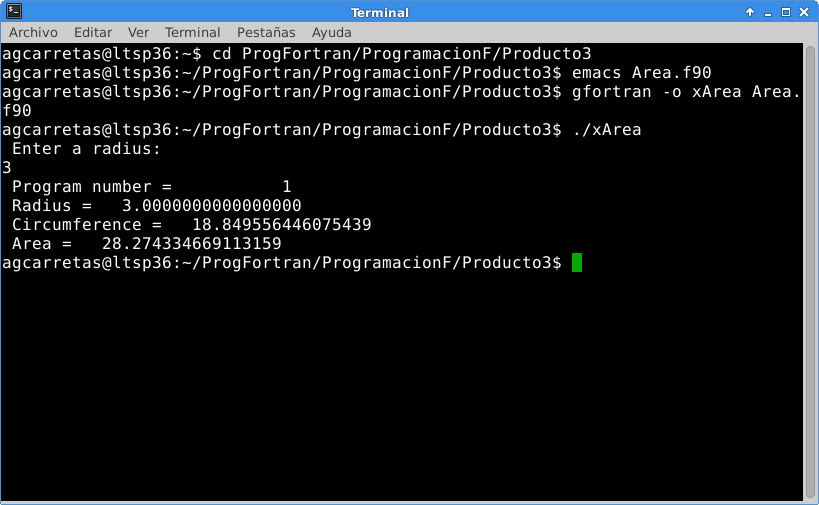
\includegraphics[width=10cm]{Area}
\end{figure}

\begin{verbatim}! Area . f90 : Calcula el area de un circulo

 Program areacirculo
  Implicit None 
   Real *8 :: radius , circum , area 
   Real *8 :: PI = 4.0 * atan(1.0)
  Integer :: model_n = 1 
   print * , 'Enter a radius:' 
   read * , radius 
  circum = 2.00 * PI * radius 
  area = radius * radius * PI 
  print * , 'Program number =' , model_n 
  print * , 'Radius =' , radius 
  print * , 'Circumference =' , circum 
  print * , 'Area =' , area 
 End Program areacirculo \end{verbatim}

\subsection{Volumen de un segmento esférico}
\begin{figure}[H]
	\centering
    \includegraphics[width=6cm]{Esfera}
\end{figure}
La imagen superior muestra gráficamente el volumen que nuestro nuevo código debería calcular. Basándonos en el código del programa anterior, nuestra tarea fue la de rediseñarlo, de manera que mostrara el resultado del volumen de un segmento esférico, teniendo como variables al radio y la altura. 

\begin{figure}[H]
	\centering
    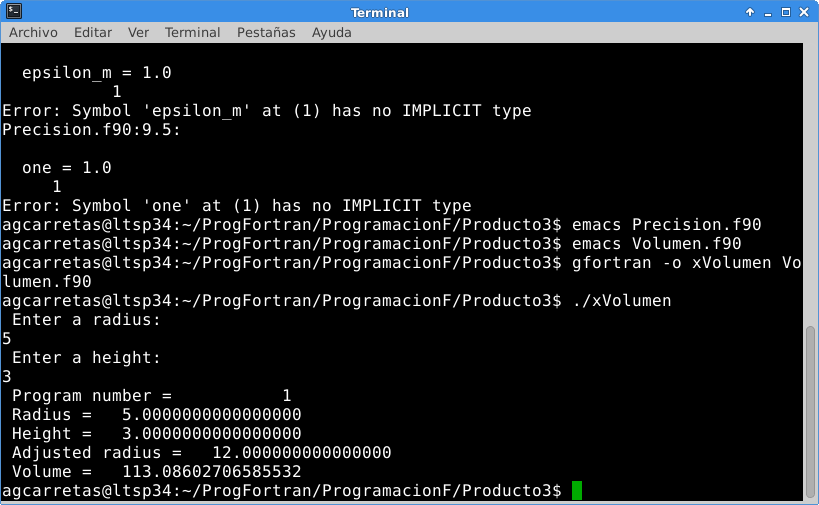
\includegraphics[width=10cm]{Volumen}
\end{figure}

\begin{verbatim}! Volumen . f90 : Calcula el volumen de una region esferica

 Program volumenregion
  Implicit None 
   Real *8 :: radius , radiusx , volume, height 
   Real *8 :: PI = 4.0 * atan(1.0)
   Integer :: model_n = 1 
   print * , 'Enter a radius:' 
   read * , radius 
   print * , 'Enter a height:'
   read * , height
  radiusx = 3.00 * radius - height
  volume = 0.3333 * PI * height * height * radiusx 
  print * , 'Program number =' , model_n 
  print * , 'Radius =' , radius 
  print * , 'Height =' , height
  print * , 'Adjusted radius =' , radiusx 
  print * , 'Volume =' , volume 
 End Program volumenregion 
\end{verbatim}

\subsection{Precisión de una máquina}
La actividad consistía en determinar la precisión de la computadora en la que se trabaja, utilizando una herramienta de precisión doble, si esta interactuaba durante sesenta ocasiones. 

\begin{figure}[H]
	\centering
    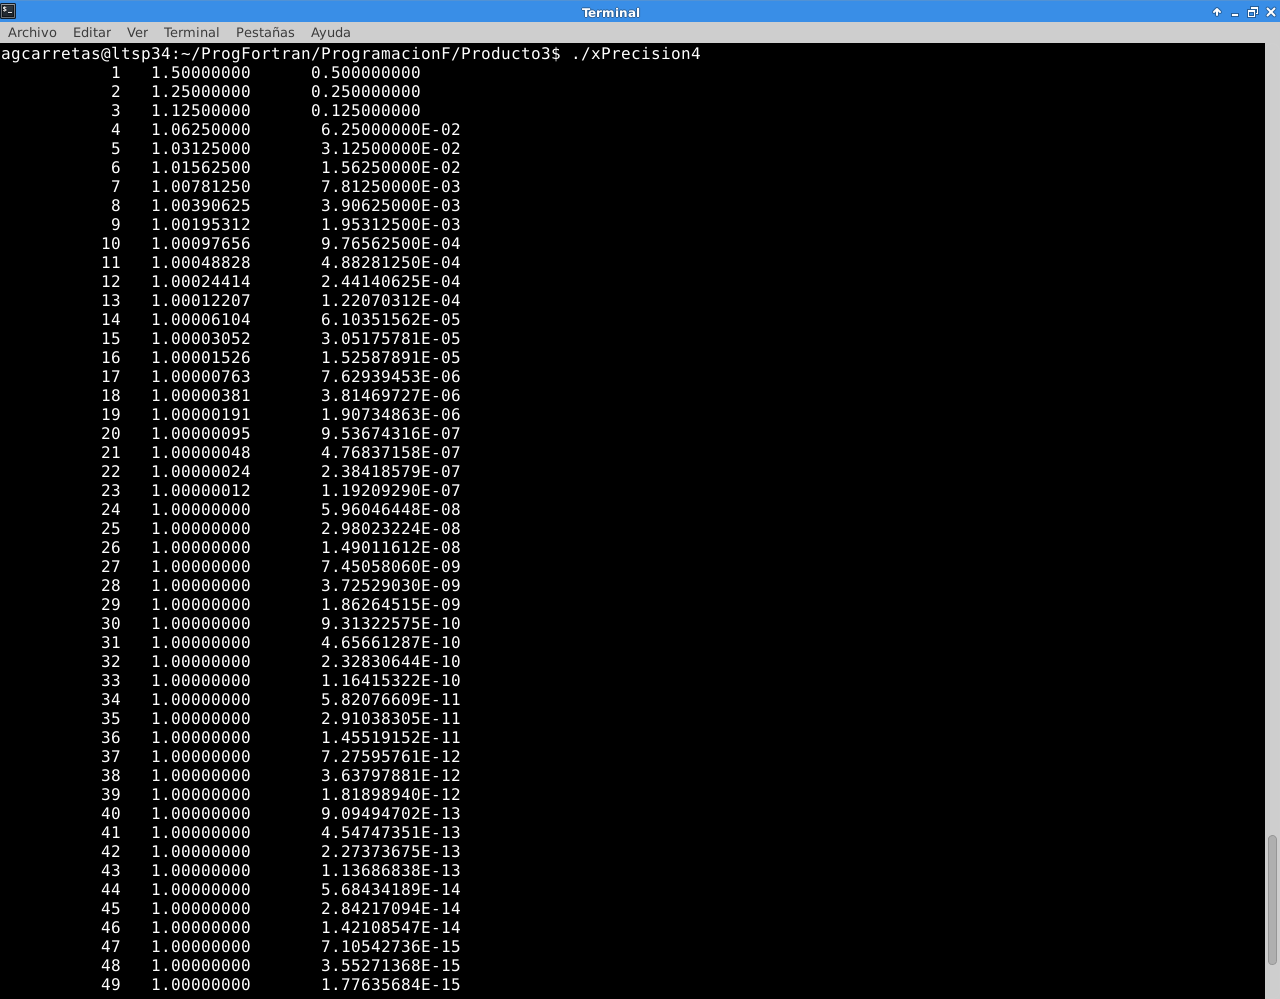
\includegraphics[height=6cm, width=10cm]{Precision}
\end{figure}

\begin{verbatim}! Precision . f90 : Determina la precision de la computadora

 Program Precision
   Implicit None
   Integer :: i , n
   Real *8 :: epsilon_m , one
   n=60 
   epsilon_m = 1.0
  one = 1.0
  
  do i = 1, n , 1 
    epsilon_m = epsilon_m / 2.0 
    one = 1.0 + epsilon_m 
    print * , i , one , epsilon_m 
  end do 
 End Program Precision\end{verbatim}

\subsection{Precisión de una máquina 2.0}
Este código fue retomado del anterior, con el simple hecho de cambiarle la precisión a sencilla.

\begin{figure}[H]
	\centering
    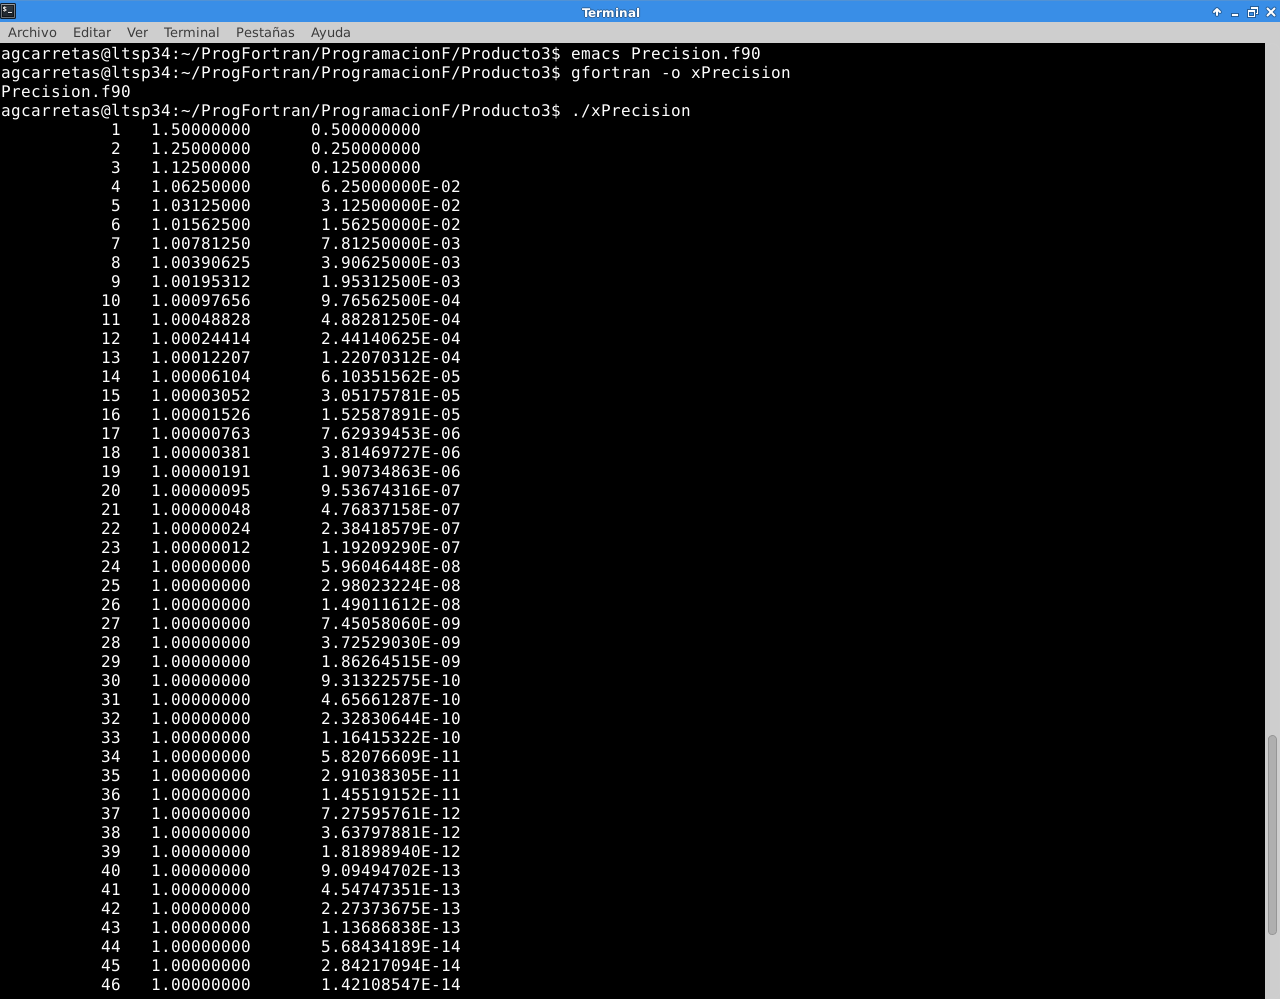
\includegraphics[height=6cm, width=10cm]{Precision4}
\end{figure}

\begin{verbatim}! Precision . f90 : Determina la precision de la computadora

 Program Precision
   Implicit None
   Integer :: i , n
   Real *8 :: epsilon_m , one
   n=60 
   epsilon_m = 1.0
  one = 1.0
  
  do i = 1, n , 1 
    epsilon_m = epsilon_m / 2.0 
    one = 1.0 + epsilon_m 
    print * , i , one , epsilon_m 
  end do 
 End Program Precision\end{verbatim}

\subsection{Funciones matemáticas}
El objetivo era el exponer por medio de variables, que \textbf{FORTRAN} tiene ciertas funciones matemáticas predefinidas. Se calcularon ciertos valores senoidales y exponenciales.

\begin{figure}[H]
	\centering
    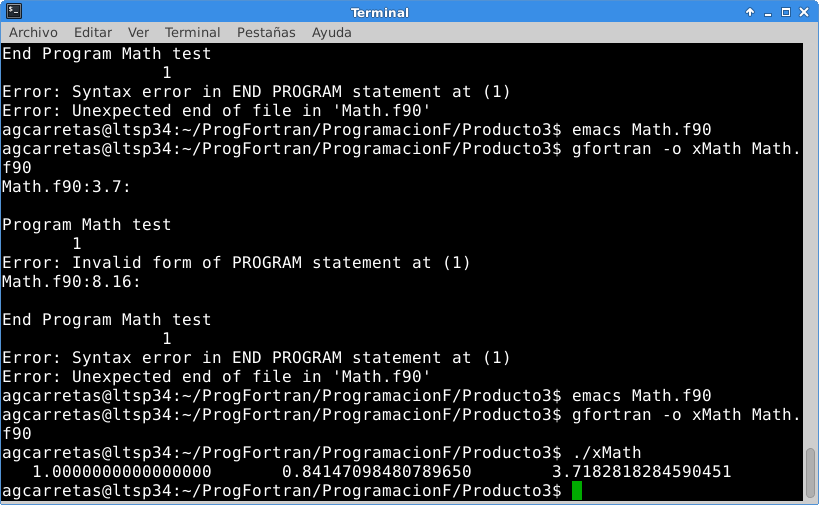
\includegraphics[width=10cm]{Math}
\end{figure}

\begin{verbatim}! Math . f90 : demo de algunas funciones matematicas en Fortran

Program Mathtest 
  Real *8 :: x = 1.0 , y, z 
  y = sin (x) 
  z = exp (x) + 1.0 
  print * , x, y, z 
End Program Mathtest 
\end{verbatim}

\subsection{Otro tipo de funciones matemáticas}
Continuando con expresiones matemáticas predefinidas, se presentaron como operaciones que manejaban resultados en los complejos. O infinitos.

\begin{figure}[H]
	\centering
    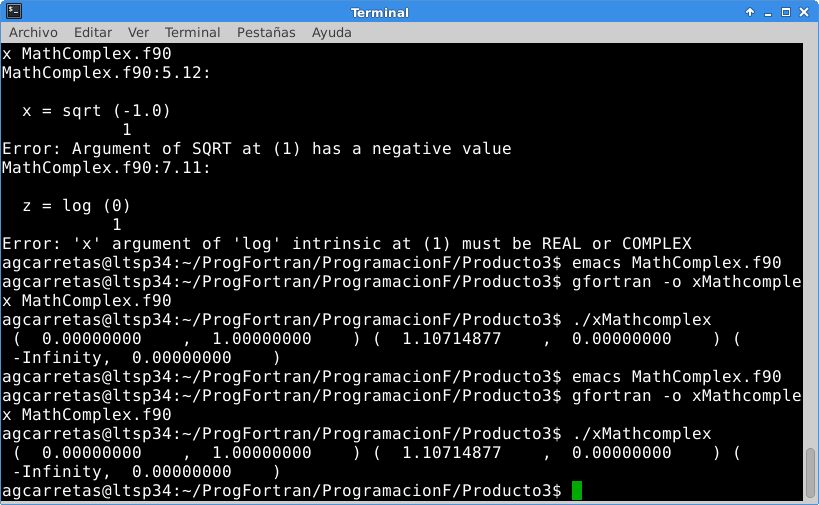
\includegraphics[width=10cm]{Mathcomplex}
\end{figure}

\begin{verbatim}! Mathcomplex . f90 : demo de algunas funciones matematicas en Fortran

Program Mathcomplex 
  Complex *8 :: x = -1.0 , y = 2.0 , z = 0 , xx , yy , zz
  xx = sqrt (x) 
  yy = atan (y) 
  zz = log (z)
  print * , xx, yy, zz 
End Program Mathcomplex\end{verbatim}

\subsection{Declarando nuevas funciones}
Declaramos una función que denotaba cierta trigonométrica dependiendo de dos variables, que las introducirá el usuario. Después, se incluyó esa función en un programa que calculaba valores influenciados por la anterior función propuesta.

\begin{figure}[H]
	\centering
    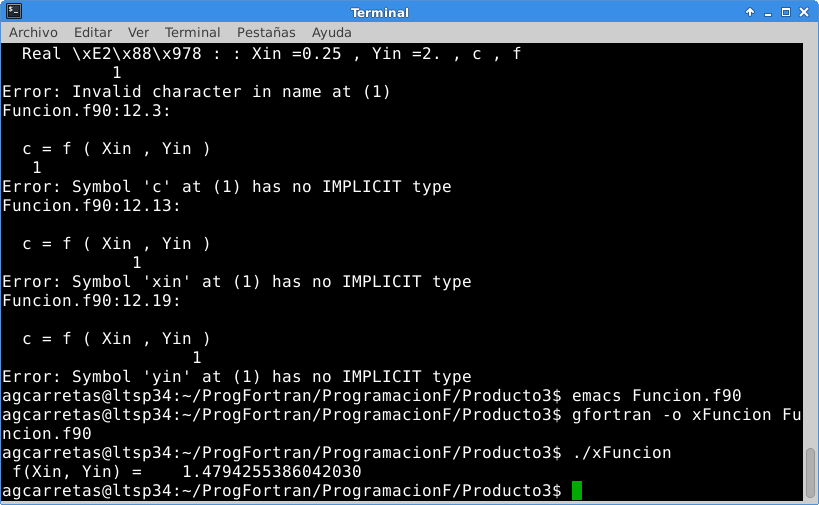
\includegraphics[width=10cm]{Funcion}
\end{figure}

\begin{verbatim}! Funcion . f90 : Creando funciones

 Real *8 Function f (x,y)
   Implicit None
   Real *8 :: x, y
   f = 1.0 + sin (x*y )
 End Function f
 
 Program Main
  Implicit None 
  Real *8 :: Xin =0.25 , Yin =2. , c , f 
  c = f ( Xin , Yin )
  write ( * , * ) 'f(Xin, Yin) = ' , c
 End Program Main\end{verbatim}

\subsection{Subrutinas}
Las subrutinas son subprogramas que no devuelven ningún resultado, por tanto no tienen tipo. Las subrutinas son una herramienta de FORTRAN para simplificar el trabajo, pues llama a elementos de otras funciones, y les agrega más información cada que son utilizadas.

\begin{figure}[H]
	\centering
    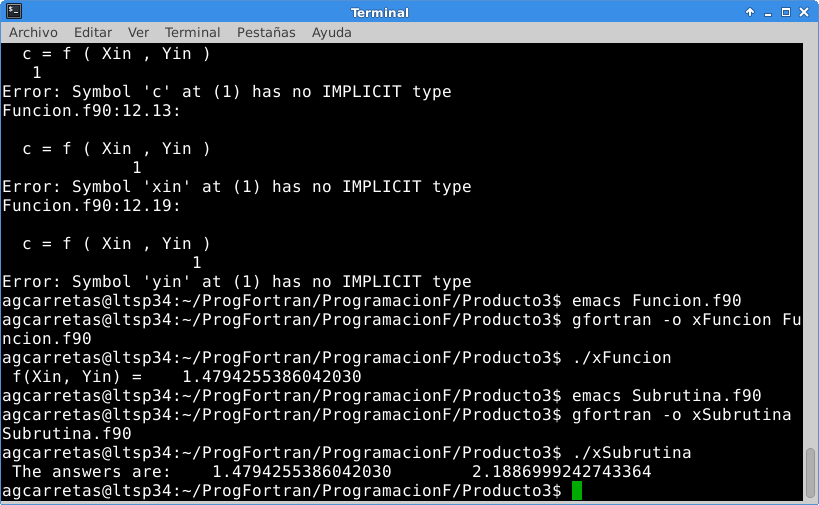
\includegraphics[width=10cm]{Subrutina}
\end{figure}

\begin{verbatim} ! Subrutina . f90 : Demuestra la llamada de una subrutina

 Subroutine g(x, y, ans1 , ans2 )
   Implicit None
   Real (8) :: x , y , ans1 , ans2 
   ans1 = sin (x*y) + 1.
   ans2 = ans1**2
 End Subroutine g
 
 Program Mainprogram 
   Implicit None
   Real *8 :: Xin =0.25 , Yin =2.0 , Gout1 , Gout2
   call g( Xin , Yin , Gout1 , Gout2 ) 
   write ( * , *) 'The answers are: ' , Gout1 , Gout2
End Program Mainprogram 
\end{verbatim}

% Nunca debe faltar esta última linea.
\end{document}